\section{Modulación pasabanda binaria y su espectro de potencia}
%
%Al igual que en el caso de banda base, comenzamos el estudio de estas formas de onda
%analizando la densidad espectral de potencia correspondiente.

\subsection*{Modulación pasabanda binaria lineal}

Consideramos aquí la onda
\[
x_c(t) = \sum_k a_k p(t-kT_s) \cos(\omega_c t),
\]
donde los símbolos $\{a_k\}$ son I.I.D., binarios. Esta se\~nal puede interpretarse
como el resultado de una modulación analógica en banda lateral doble (DSB) aplicado a la onda PAM de banda base $x(t) = \sum_k a_k p(t-kT_s)$.
El caso de ASK corresponde a una onda PAM unipolar, mientras que el de BPSK corresponde a la polar.

\newpage

Podemos utilizar esta identificación para obtener la densidad espectral de potencia de la onda modulada:

\begin{equation}
    \label{eq:dep}
    \col{S_{x_c}(f) = \frac{S_x(f-f_c) + S_x(f+f_c)}{4}}\tag{\#}
\end{equation}

\noindent donde recordamos la expresión para la densidad espectral de potencia en banda base:
\[
S_x(f) = \sigma_a^2 f_s |\hat{P}(f)|^2 + \mu^2 f_s^2 \sum_{n=-\infty}^{+\infty} |\hat{P}(n f_s)|^2\delta(f-nf_s).
\]
Aquí $\mu$ y $\sigma_a^2$ son la media y varianza, respectivamente, de los símbolos I.I.D. $\{a_k\}$, y \\ $\hat{P}(f)$ la
transformada de Fourier del pulso de banda base.


\paragraph{Comentario.} En rigor, para justificar esta fórmula a partir de los procesos estacionarios había que introducir
un retardo aleatorio en la onda PAM, y también para obtener (\ref{eq:dep}) de la modulación DSB se incluía una fase aleatoria.
Ignoramos estos temas de aquí en mas, interpretando las densidades
espectrales en el sentido de las señales determinísticas de
potencia finita.


\subsubsection*{Caso de modulación BPSK}

La onda pasabanda BPSK $x_c(t)$ corresponde a modular una onda PAM de banda base $x(t)$ {\em polar, binaria}, con $a_k=\pm A$. Recordemos que ésta tiene densidad espectral de potencia $S_x(f)= A^2 f_s |\hat{P}(f)|^2$. Bosquejamos la correspondiente $S_{x_c}(f)$ en dos casos particulares.

\begin{minipage}{0.5\textwidth}
\begin{enumerate}
    \item Pulsos de Nyquist con exceso de ancho de banda $\alpha$

    $\hat{P^1}(f) = $\parbox[m]{0.6\textwidth}{\resizebox{0.6\textwidth}{!}{
            \bpgf{Imagenes/MDPasa/MDPasa-5}
            \begin{tikzpicture}
                \draw [-stealth] (-2,0) -- (2,0) node [anchor=north] {$f$};
                \draw [-stealth] (0,-0.5) -- (0,2);
                \draw [samples=200,domain=-1.25:-0.75] plot (\x,{1/2*(1+cos(2*pi*(\x-0.25) r))}) -- (0.75,1);
                \draw [samples=200,domain=0.75:1.25] plot (\x,{1/2*(1+cos(2*pi*(\x+0.25) r))});
                \path (0,1) node [anchor=south west] {$T_s$};
                \draw [dotted] (1,0.5) -- (1,0) node [anchor=north] {$\frac{f_s}{2}$};
                \draw [dotted] (-1,0.5) -- (-1,0) node [anchor=north] {$-\frac{f_s}{2}$};
            \end{tikzpicture}
            \endpgfgraphicnamed}}

    \item Pulsos NRZ, $\hat{P^2}(f) = T_s \sinc (\pi T_s f)$.
\end{enumerate}
\end{minipage}\hfil
\begin{minipage}{0.45\textwidth}
    \resizebox{\textwidth}{!}{
    \bpgf{Imagenes/MDPasa/MDPasa-6}
    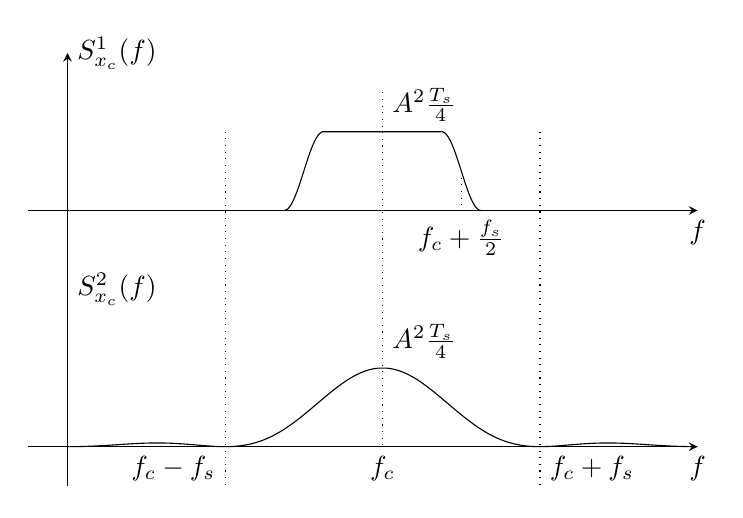
\begin{tikzpicture}
        \draw [-stealth] (-0.5,0) -- (8,0) node [anchor=north] {$f$};
        \draw [-stealth] (0,-3.5) -- (0,2) node [anchor=west] {$S^1_{x_c}(f)$};
        \path  (0,-1) node [anchor=west] {$S^2_{x_c}(f)$};
        \begin{scope}[shift={(4,0)}]
                    \draw [samples=200,domain=-1.25:-0.75] plot (\x,{1/2*(1+cos(2*pi*(\x-0.25) r))}) -- (0.75,1);
                    \draw [samples=200,domain=0.75:1.25] plot (\x,{1/2*(1+cos(2*pi*(\x+0.25) r))});
                    \path (0,1) node [anchor=south west] {$A^2\frac{T_s}{4}$};
                    \draw [dotted] (1,0.5) -- (1,0) node [anchor=north] {$f_c+\frac{f_s}{2}$};
        \end{scope}
        \begin{scope}[shift={(0,-3)}]
            \draw [-stealth] (-0.5,0) -- (8,0) node [anchor=north] {$f$};
            \draw [samples=210,domain=0:8] plot (\x,{(sin(pi/2*(\x-4) r)/(pi/2*(\x-4)))^2});
            \path (4,1) node [anchor=south west] {$A^2\frac{T_s}{4}$};
        \end{scope}
        \draw [dotted] (2,1) -- (2,-3) node [anchor=north east] {$f_c-f_s$} -- (2,-3.5);
        \draw [dotted] (6,1) -- (6,-3) node [anchor=north west] {$f_c+f_s$} -- (6,-3.5);
        \draw [dotted] (4,1.5) -- (4,-3) node [anchor=north] {$f_c$};
    \end{tikzpicture}
    \endpgfgraphicnamed}
\end{minipage}

El segundo caso ocupa una banda mucho mayor (en principio,
infinita). En general se utiliza algún criterio práctico que considera un ancho de banda efectivo
para esos casos. Por ejemplo, considerar solamente el ``lóbulo central'' de la densidad espectral,
que tiene $90\%$ de la potencia.
\FloatBarrier

\subsubsection*{Caso ASK, pulsos NRZ}$\phantom{1}$

\begin{figure}[htb]
    \centering\begin{minipage}{\textwidth}
    \bpgf{Imagenes/MDPasa/MDPasa-7}
    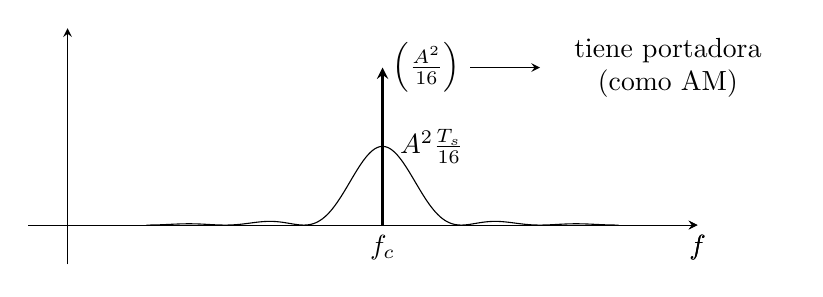
\begin{tikzpicture}
        \draw [-stealth] (-0.5,0) -- (8,0) node [anchor=north] {$f$};
        \draw [-stealth] (0,-0.5) -- (0,2.5);
        \draw [-stealth] (-0.5,0) -- (8,0) node [anchor=north] {$f$};
        \draw [samples=210,domain=1:7] plot (\x,{(sin(pi*(\x-4) r)/(pi*(\x-4)))^2});
        \path (4.1,1) node [anchor=west] {$A^2\frac{T_s}{16}$};
        \draw [thick,-stealth] (4,0) node [anchor=north] {$f_c$} -- (4,2) node (a) [anchor=west] {$\left(\frac{A^2}{16}\right)$};
        \node [anchor=west] (b) at (6,2) {\parbox{3cm}{\centering tiene portadora (como AM)}};
        \draw [-stealth] (a) -- (b);
    \end{tikzpicture}
    \endpgfgraphicnamed\end{minipage}
\end{figure}
\FloatBarrier

La combinación de ASK con pulsos de Nyquist es en principio
también posible, pero no de uso práctico ya que ASK se motiva
principalmente por razones de simplicidad.


%\newpage

\subsection*{Modulación FSK binaria}

\begin{minipage}{0.5\textwidth}
\[x_c(t) = \sum_k A p(t-kT_s)\cos (\omega_c t + 2\pi f_k t),\]
donde $f_k=\pm f_\Delta$, y los pulsos son NRZ.
\end{minipage}
\hfil
\begin{minipage}{0.45\textwidth}
    \resizebox{\textwidth}{!}{
    \bpgf{Imagenes/MDPasa/MDPasa-10}
    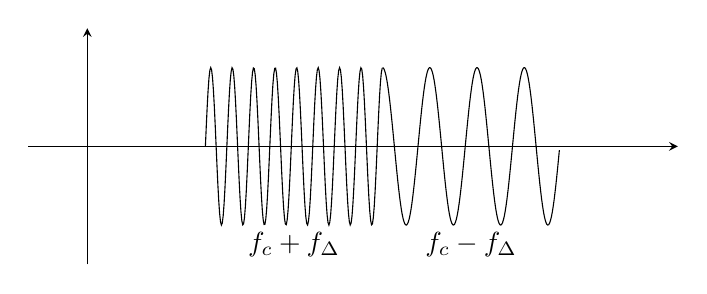
\begin{tikzpicture}[xscale=1.5]
        \draw [-stealth] (-0.5,0) -- (5,0);
        \draw [-stealth] (0,-1.5) -- (0,1.5);
        \draw [domain=1:2.5,samples=200] plot (\x,{-sin(pi*\x r + 10*pi*\x r)});
        \draw [domain=2.5:4,samples=200] plot (\x,{sin(pi*\x r + 4*pi*\x r)});
        \path (1.75,-1.25) node {$f_c+f_\Delta$};
        \path (3.25,-1.25) node {$f_c-f_\Delta$};
    \end{tikzpicture}
    \endpgfgraphicnamed}
\end{minipage}

Notar que la onda FSK puede verse como la superposición de dos ondas ASK,
una en cada frecuencia, activadas por los símbolos opuestos.
?`Es posible evaluar su espectro de potencia superponiendo los de ASK?
Esto no esta justificado ya que las ondas ASK no son independientes, pero nos
sirve para tener una idea:

\begin{figure}[htb]
    \centering\begin{minipage}{\textwidth}
    \bpgf{Imagenes/MDPasa/MDPasa-11}
    \begin{tikzpicture}[xscale=1.5]
        \draw [-stealth] (-0.5,0) -- (8,0) node [anchor=north] {$f$};
        \draw [-stealth] (0,-0.5) -- (0,2.5);
        \draw [samples=400,domain=1:7] plot (\x,{2*(sin(2*pi*(\x-3) r)/(2*pi*(\x-3)))^2+2*(sin(2*pi*(\x-5) r)/(2*pi*(\x-5)))^2});
        \draw [-stealth,thick] (3,0) node [anchor=north] {$f_c-f_\Delta$} -- (3,2.3);
        \draw [-stealth,thick] (5,0) node [anchor=north] {$f_c+f_\Delta$} -- (5,2.3);
    \end{tikzpicture}
    \endpgfgraphicnamed\end{minipage}
\end{figure}
\FloatBarrier


\noindent La evaluación rigurosa del problema no es sencilla (recordar que tampoco era sencillo evaluar espectros de FM).
Un caso resuelto por Sunde (ver libros) es para
$f_\Delta=\frac{f_s}{2}$. El resultado tiene la forma (\ref{eq:dep}), trasladando el espectro pasabajos

\begin{minipage}{0.6\textwidth}
\begin{align*} S_{x}(f) =& \frac{A^2}{4}\left[\delta(f-\frac{f_s}{2})+\delta(f+\frac{f_s}{2})\right]\\& + \frac{4 A^2 T_s \cos^2(\pi T_s f)}{\pi^2 (4 T_s^2 f^2 - 1)^2}.\end{align*}
\end{minipage}\hfil
\begin{minipage}{0.4\textwidth}
    \resizebox{\textwidth}{!}{
%\begin{figure}[htb]
%    \centering
    \bpgf{Imagenes/MDPasa/MDPasa-12}
    \begin{tikzpicture}[xscale=1.5]
        \draw [-stealth] (-3,0) -- (3,0) node [anchor=north] {$f$};
        \draw [-stealth] (0,-0.5) -- (0,2.5);
        \draw [samples=400,domain=-2.5:2.5] plot (\x,{20*(cos(pi*\x r)/(pi*(4*\x^2-1)))^2});
        \draw [-stealth,thick] (-0.5,0) node [anchor=north] {$-\frac{f_s}{2}$} -- (-0.5,2.3);
        \draw [-stealth,thick] (0.5,0) node [anchor=north] {$\frac{f_s}{2}$} -- (0.5,2.3);
        \draw (-1.5,0.1) -- (-1.5,-0.1) node [anchor=north] {$-3\frac{f_s}{2}$};
        \draw (1.5,0.1) -- (1.5,-0.1) node [anchor=north] {$3\frac{f_s}{2}$};
    \end{tikzpicture}
    \endpgfgraphicnamed}
%\end{figure}
\end{minipage}

%

Concluimos que la onda FSK ocupa un ancho de banda algo mayor que las modulaciones lineales ASK, BPSK, una vez más en
forma consistente con la situación en las modulaciones analógicas correspondientes.




\subsection*{Sobre eficiencia espectral en modulación digital
pasabanda}

Notar que en todas las modulaciones consideradas el ancho de banda
es como mínimo el doble que la correspondiente situación de banda base.
Ello implica que la eficiencia espectral en bps/Hz será la mitad.

Por ejemplo, si usamos BPSK con pulsos ideales de Nyquist, ocupa una banda $f_s$,
y obtiene una eficiencia espectral igual a 1, comparado con 2 en el caso de banda base.

La forma de compensar esto es enviando más bits por símbolo, es decir para a modulaciones $M$-arias;
las estudiamos a continuación.
